\section{Initial proof-of-concept realisation}  \label{eq:realisation}


\subsection{Background notions: Blockchain and Smart Contract}  \label{sec:blockchain}
Blockchain is essentially a distributed ledger of information (e.g., a transaction from A to B in the bitcoin world), a copy of which cannot be arbitrarily altered without being spotted and for which consistency of each information can be achieved through a decentralized and distributed consensus, without requiring trust in any third party but instead, through large and flat pool of so-called miners using cryptographic primitives [add reference to satoshi paper].
Blockchain has been later leveraged to manage Smart Contracts, small pieces of software that encode a set of conditions and actions that a machine can interpret and that can be executed as expected using the blockchain infrastructure without third party involvement or supervision [18]. Smart contracts represent therefore a well-suited decentralized tool to implement Traffic Cube and Settlement functionalities. Being one of the most adopted and well-supported by the developer community, we decide to use Ethereum Smart Contract implementation.

In the Ethereum network, any node uses a virtual machine (EVM), which can execute code of arbitrary algorithmic complexity, to execute smart contracts, the integrity of whose is always guaranteed. A smart contract can perform various state updates and account balancing.  
Executing a smart contract results in one or more transactions to be validated. Each transaction has a cost (e.g., fee) associated, which translates into incentive for any miner within the network to independently execute it. 
More specifically, any operation being performed within a transaction consumes a fixed amount of Gas. Miners fees are therefore proportional to the amount of Gas used. Gas price is measured in terms of Ether (the Ethereum cryptocurrency). Every transaction specifies the gas price a smart contract is willing to pay for its execution, thus, the total fee paid for a transaction is the result of Gas amount multiplied by the Gas selected price.


\note{cite in blockchain section}

\note{	\cite{Swan}  Swan, M. (n.d.). Blockchain : blueprint for a new economy.}

\note{\cite{Buterin2014} Buterin, V. (2014). A next-generation smart contract and decentralized application platform. Retrieved from http://buyxpr.com/build/pdfs/EthereumWhitePaper.pdf}


%The second element of our approach is based on the use of emergin Blockchain and Smart Contracts tecnhology.

%\note{FIXME -- still a dump of Michele's text . background}

%Blockchain is essentially a distributed ledger of information (e.g., a transaction from A to B in the bitcoin world), a copy of which cannot be arbitrarily altered without being spotted and for which consistency of each information can be achieved in a decentralized and distributed way, without requiring trust in any third party. These properties, that in the bitcoin world provides a very strong business case (e.g., removing transaction costs associated to clearinghouse functionalities when transferring money), can also provide a trust case for exchanging access to different assets, without requiring trust among parties.

%Decentralized Applications (DApps) use assets and services from different sources, not controlled by only one entity (in contrast to the traditional centralized client/server web). Using smart contracts and off-chain information makes more practical to develop new DApps. s-Health apps can be seen as a particular type of DApps. Bitcoin is the first DApp built on top of the blockchain: it is a digital and interoperable currency (i.e., it does not require conversion across the world), using the blockchain infrastructure and some complex cryptographic algorithms, to achieve (nearly) zero transaction fees while avoiding the double-spending problem (e.g., possibility to spend a given amount twice) and without requiring to trust in any third party to police this risk. Thinking about the value of different assets, bitcoin and alt-coin (i.e., bitcoin plus metadata) can provide an interoperable and open cross-domain incentives platform for redistributing the value created from assets sharing, transparently covering the interests of all the involved assets providers.

%Blockchain has been later leveraged to manage Smart Contracts, small pieces of software that encode a set of conditions and actions that a machine can interpret and that can be executed as expected using the blockchain infrastructure without third party involvement or supervision \cite{Buterin2014}. These functionalities can be interesting when it comes to give permission to access different assets (datasets and devices) only for specific purposes.

%Blockchain is usually adopted by Decentralized Autonomous Organizations (DAOs), which require neither written statements nor physical governance bodies, to run on code expressed by a set of Smart Contracts. This concept is interesting for organizations where different stakeholders can vote and agree on the rules for sharing their assets, e.g., for particular social benefits or research purpose, thus deciding how their rewards should be distributed while influencing and supporting the creation of specific s-Health services. Through DAOs, the principles, rules and benefits deriving from data sharing can be distributedly enforced without requiring any trusted third party. While this is a powerful concept to achieve autonomy and avoid misuse, particular attention is required in order to properly encode the right human assisted governance structure in the DAOs. This might require a governance body that supervises the rules implemented as DAO by an open developers community, following a rigorous, open, transparent and accounted review process.


%\note{ANDREA}


%\authornote{We need reference to ETH architecture, with APIs call and a snippet of the code. We can add some numbers on how much this will cost to run and consequently set up a minimum cost for each data in order to keep infrastructure sustainable.
%Logic: “data” is a “count cube”. The platform generates a stream of these cubes at a certain rate, which is tunable using the window size on the TrackerDB. The arrival rate of the cubes determines the frequency at which contracts are executed, and therefore the cost over time.
%}
\subsection{Implementation}
The generation of unilateral cubes can rely on different implementation choices made within the Data Producers (DP) and VAS Trusted Zones. This doesn’t affect the properties of the Traffic Cube and Settlement, because liability is pushed at the edge. Section X provides some detail on how unilateral cube generation can be implemented. 
Here we instead focus on detailed implementation of the Traffic Cube and Settlement functionalities using smart contracts. 
We developed them using Solidity, the Ethereum’s scripting language. To implement the contracts we assigned an Ethereum account to each DP and VAS. We connected these accounts to our private Ethereum test network, deployed on a single node with 6-core Intel Xeon E5-2640 and 16GB of RAM. We wrote, deployed and evaluated smart contracts in the network by using the Ethereum web browser based IDE REMIX, connected to our private chain through RPC protocol. In our implementation, accounts prepare and send the transactions to the blockchain to instances of Geth through RPC. To measure gas consumption, we used the debug tool provided by Remix and we observed the difference in the account balance before and after invoking the contract to measure the transaction cost.

A limitation of Ethereum smart contracts is that they cannot directly access off-chain data about real-world state and events. In our case this represents a challenge in acquiring unilateral cubes value. More precisely, smart contracts are independently executed by any node in the chain, thus, each execution needs to retrieve such information from an off-chain source independently, without any assurance of the information integrity.
To overcome this limit, the concept of "oracle" has been introduced. Simply speaking, an oracle is a special contract that serves data requests from traditional contracts, by sourcing them from designated data feeds. 
Two options are possible for implementing oracles. The first one is relying on existing proxy services. Oraclize provides a "programmable" oracle that can interact with any datasource selected among a predefined set of standard channels. In addition Oraclize provides an authenticity proof by means of a TLSNotary proof[cite] which guarantees the authenticity and integrity of the retrieved data. These functionalities come at a cost. For each off-chain query, Oraclize requires a fee which includes a commission, ranging from 0.01\$ to 0.04\$, and a refund of the Gas used to perform the transaction. 
The other option is when each party of the contract, Data Producer and VAS, independently update their unilateral cubes by pulling their values from cubes generator located within their Trusted Zones and then creating a transaction which embeds the cubes in the blockchain. This way any node executing the smart contract will have the same copy of that cube. As a result, costs associated to the use of an external oracle service, such as Oraclize, can be saved. Because in our model responsibility and liability of producing faulty cubes is placed to Data Producers and VASs, this option well suffices to our needs.
Figure XX shows pseudo-code of our settlement contract. For the sake of simplicity, this snippet of code only accounts for the single Data Producer and the single VAS scenario, although generalization are straightforward.
The contract first requests the involved parties to provide their unilateral cubes; then it uses this information to perform the actual settlement, by combining the two unilateral cubes. If the processed combined cube is consistent then a payment to the producer is performed, otherwise, a dispute resolution mechanism should be invoked.

	\note{new from Michele}
\begin{verbatim}
	
function callback(queryID, result)\{


if (msg.sender != oraclize_cbAddress()) \{


just to be sure the calling address is the Oraclize authorized one
throw;


\}


if(queryID == firstQuery)\{


producer = result;


secondQuery = update(url, maxGas);


\}


else if(queryID == secondQuery)\{


consumer = result;


if(Compare(producer, consumer)==0)\{


transfer(producerAddress, dataPrice * result);  


\}


else dispute_resolution();

\end{verbatim}


When a dispute resolution is invoked, payments are retained from being performed due to impossibility to clearly identify the correct unilateral cube. However a reputation mechanism can be implemented in order to penalize both parties involved in a given settlement transaction and to ultimately promote honest behaviour. As it is not expected that reputation computation will require off-chain interaction~\cite{schaub2016trustless,carboni2015feedback}, we are confident that while not considering its implementation in this phase this will not significantly affect the overall contract execution costs.

\section{Evaluation and Lessons learnt}  \label{sec:evaluaton}

Aim of this section is to quantify the cost of the smart contract described above and the associated cube settlement operations. By considering the scenario in which one VAS consumes the data of one Data Producer, we evaluate how the cost of performing such contract changes depending on the number of data exchanged and the number of settlements transactions required. Considering different quantity of exchanged data reflect the different purpose of the exchange (event-based data rather than real-time series acquisition). Nevertheless the reason for considering a variation in the number of required settlement needs some clarification. The most natural strategy will be to perform the settlement at the end of each contractually agreed data exchange, however in the early stage of an hypothetical market place where new producers and VASs join without necessarily trusting each other nor having an already established reputation, two situations might occur:
\begin{itemize}
	\item {Data producers and VASs have low reputation hence their trust level is low and the risk of claiming wrong unilateral cubes high. In this case, by performing more than one cube settlement, in an initial rump-up phase of a given data exchange will allow them to mutually increase their reputation and trust;}
	\item {Data producers and VASs have already high reputation hence they are expected to act honestly. In this case cube settlements may occur with a lower rate, eventually only at the end of a data exchange phase, because the risk of producing faulty cubes is mitigated.}
\end{itemize}
%1- 
%2- 

By evaluating the cost of performing the settlement operations we are able to define the minimum price that VASs should pay for each consumed data in order to sustain the settlement infrastructure and eventually generate profit for the Data Producers.

We define the minimum data price as the amount of Ether needed to at least cover the cost of contract deployment and transactions for performing cubes settlement operations. This means that if a producer sells data at the minimum price, its profit will be zero. 
At the time of writing one Ether costs 220\$, however, its price is still very volatile as shown in Figure [eth price].

\begin{figure}
	\centering
	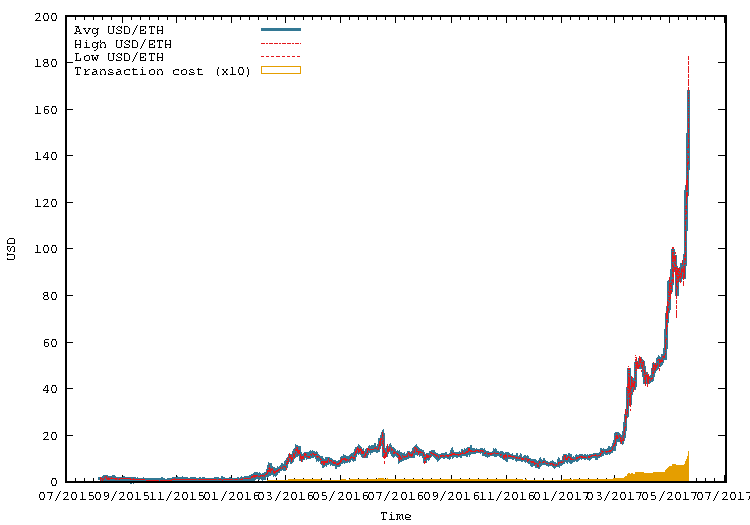
\includegraphics[width=\columnwidth]{figures/price}
	\caption{Ether price chart}
\label{fig:EthPrice}
\end{figure}

As result, transaction cost may frequently vary, thus leading to uncertainty about the economic feasibility of a specific application. We analysed the capability of Ethereum to support a stable transaction cost by tuning the Gas price. The main drawback when setting a low gas price is the increase of time required before a transaction is validated. Assuming a range of gas price between 0.9 Gwei and 20 Gwei (0.0000000009 and 0.00000002 Ether respectively), as minimum and average reported by the Ethereum network in 2017, the time required for a transaction to be validated in the chain varies from 2 minutes to 14 seconds\footnote{https://etherscan.io/chart}. As explained before, even in the case of multiple settlements, we don’t expect that meaningful data exchange will last less than 2 minutes, thus we consider a viable choice to select the current minimum Gas price.


Figure 2 shows a general overview of the minimum data price by varying the frequency of cubes clearance operations and the amount of transferred data. The price is directly proportional to the increase of the number of cubes settlement performed while inversely proportional to the increase of data amount exchanged. Clearly, the more the data a VAS purchases, the less impacts the cost of performing cubes settlement. Depending on the type of data exchanged and trustworthiness of involved parties using this figure clearly shows how an optimal settlement strategy can always be found to dynamically adapt the number of settlement operations.

\begin{figure}
	\centering
	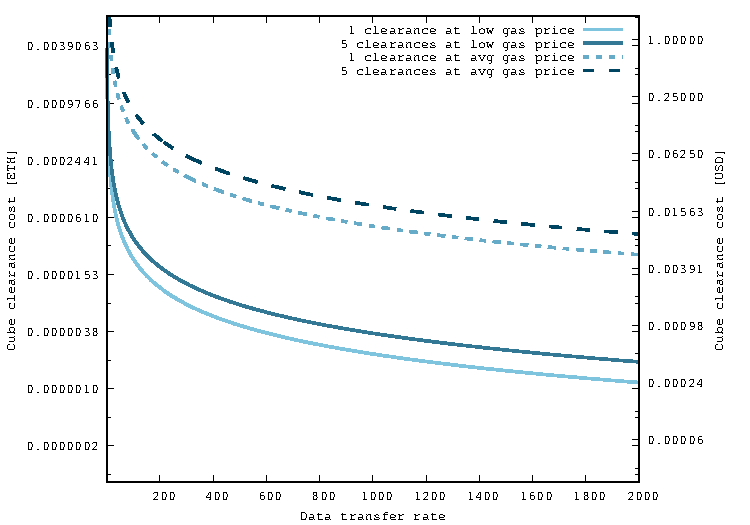
\includegraphics[width=\columnwidth]{figures/resultOraclize2-eps-converted-to}
	\caption{Without Oraclize}
	\label{fig:noOraclize}
\end{figure}

\begin{figure}
	\centering
	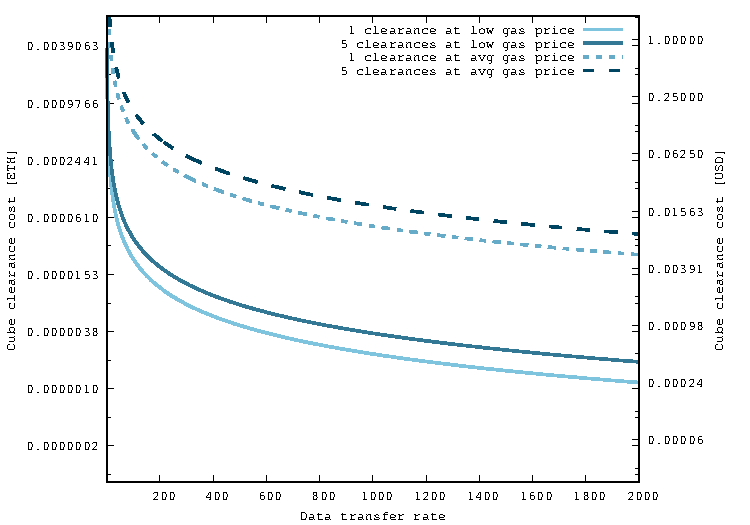
\includegraphics[width=\columnwidth]{figures/resultOraclize2-eps-converted-to}
	\caption{With Oraclize}
	\label{fig:withOraclize}
\end{figure}

Figures XXX show the total cost of performing 1 or 5 cubes settlement operations for a fixed amount of transferred data, when considering a gas price ranging from 0.9 Gwei to 20 Gwei.
More specifically, figure XXa shows the case when each party of the contract use its oracle implementation, while figure XXb shows the case when Oraclize functionalities are used. 
It worth noticing the large costs increase (on average 4 times more), due to the commission and refund of the Gas used to perform the transaction to be paid to Oraclize. 
Without Oraclize, the cost of a single cube settlement transaction ranges from 0.000099 Ether to 0.0022 Ether when the gas price selected is 0.9 Gwei and 20 Gwei respectively. The more amount of data is transferred, the less impact the transaction cost has per single data. In fact, when performing a cube settlement operation spread over 2000 data, its cost ranges from 0.00000012 Ether to 0.0000028 Ether. Alternatively, when performing 5 cube settlement over 2000 data, their cost ranges from 0.0000003 Ether to 0.000007 Ether.

\note{Add oraclize graph description}

In order to derive a profitable data price, we can consider two examples: 1) an air quality monitoring application running on a Low Power Wide Area Network (LPWAN), such as Lora, that generates data every hour, resulting in 24 measurements per day; 2) a heart rate monitoring application (e.g., fitbit), with sampling frequency of 1 second, 1 minute.  
Assuming that the cost of performing settlement operations has to be equal to 2\% of the price for that data amount.and that only one cube settlement is performed per day, Table X shows that data price ranges from 0.000001\$ to 0.00028\$ depending on the gas price selected. 
Table XXX shows estimated data price for different use cases, such as a heart rate monitoring application (e.g., fitbit), with sampling frequency of 1 second, 1 minute and 1 hour.   



%\authornote{
%\note{new from Michele}
%
%	\begin{itemize}
%\item test assuming no need of settlement, value are the same
%\item Test different time periods for cube generation, fine grained vs to larger interval, up to daily
%\item Invariance wrt to period for cube computation 
%\item Dependency wrt to number of sources and VAS (not addressed here)
%	\end{itemize}
%}
%
%
%\authornote{
%\note{old list}
%	\begin{itemize}
%		\item Are smart contracts an adequate implementation model to realise a fair marketplace?
%\item Are there limitations in the reconciliation phase?
%\item Cost of operating and marketplace: executing transactions and how to control them -- contract activated in an adaptive mode.  Who owns the contracts?  (ideal answer: nobody. Participants share the cost of transactions)
%\item Scalability: how the cubes decouple the data flow rates from the transaction frequency
%\item Data marketplace model is preliminary and not validated on real world use cases. It is based on minimal data semantics (ie the topic) and has no notion of more sophisticated contract models.
%	\end{itemize}
%}
%
%
%\authornote{
%\note{lessons learnt}
%
%	\begin{itemize}
%\item event vs time series, costs and requirements
%\item Liability of oracolize model for trust; requirements of new interfaces
%\item Volatility of market and price
%	\end{itemize}
%}
